\chapter{数据}
\section{数据来源}
\subsection{比特币数据}
\par{
    
    本文主要采用期权交易所LedgerX(https://www.ledgerx.com)公开的每日交易数据,数据位于其网站上(data.ledgerx.com),该交易所的所有期权均为欧式期权。数据包括期权合约条款(行权价、是否为认购、到期日)、每日成交量加权平均价、成交量、持仓量、最后一次买价和卖价等。其中一天的数据示例如下图所示:
    \begin{figure}[H]
        \begin{small}
            \begin{center}
                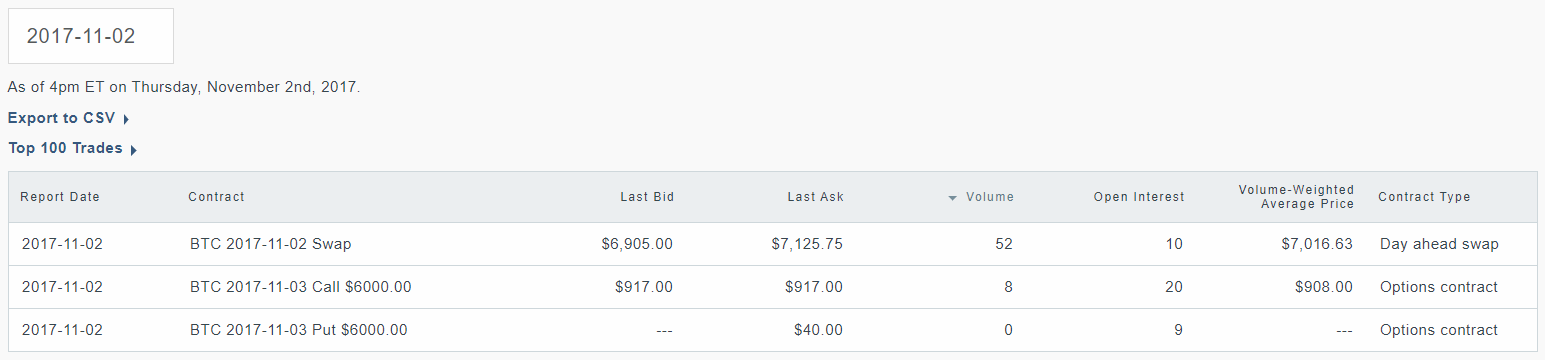
\includegraphics[width=0.95\textwidth]{figures/data_example.png}
            \end{center}
            \caption{LedgerX数据展示}
            \label{data_example}
        \end{small}
    \end{figure}
    利用python爬虫获取了2017年10月17日至2018年12月31日的全部数据,剔除了如图\ref{data_example}中所示的隔夜互换、交易量为0(只有买价或卖价)的数据之后,得到共计1726条期权的交易数据。
}
\subsection{比特币数据}
\par{
    比特币有众多交易所,根据前述参考文献可知,不同交易所之间价格存在一定差异,且用不同正常货币交易的交易所之间套利空间更为巨大\cite{Makarov-2018},因此这里我们限制选择以美元为交易货币的交易所,根据比特币数据汇总网站Bitcoinity(https://bitcoinity.org)提供数据,可得到所有美元交易所中,每日结算价中最高者和最低者之比,这一比值走势如下图:
    \begin{figure}[H]
        \begin{small}
            \begin{center}
                \includegraphics[width=0.95\textwidth]{figures/maxmin_ratio_plot.png}
            \end{center}
            \caption{交易所间最高价与最低价之比}
            \label{maxmin_ratio}
        \end{small}
    \end{figure}
    }
    \par{从图中可见交易所之间的价格差异在18年初较大,为保证之后回归的准确和套利策略的可行性,我们选择coinmarketcap网站(https://coinmarketcap.com)上公开的各大美元交易所的比特币加权均价,这样可以保证以交易量较大的比特币交易所价格为基础,位于最高者和最低者之间。
    }
\subsection{比特币无风险利率信息}
    \par{各种期权定价模型均需要有无风险利率信息,而比特币市场上并无公开的无风险利率。根据2015年出版的《比特币手册(Bitcoin Handbook)》\cite{WESNER2015223},作者提出了通过宏观经济理论推断比特币无风险利率的方法,根据其提供的结果,可得比特币的无风险利率在4$\%$~6$\%$之间,考虑到利率本身对定价结果影响较小,故取比特币无风险利率为5$\%$。
    }

\section{数据描述}
    \par{
        对数据搜集期比特币每日收盘价数据取对数收益率,按照30天滚动窗口计算其波动率、偏度、峰度\footnote{考虑到比特币市场在18年初开始变动巨大,采用更长期的窗口可能不能准确反映投资者观察到的波动率信息。}。对其描述性统计如下:}

        \begin{threeparttable}[H]
            
            \centering
            \caption{比特币数据描述性统计}
            \label{btc_describe}
            \begin{tabular}{lrrrrr}
\toprule
{} &             成交量 &   对数收益率 &     波动率 &      偏度 &      峰度 \\
\midrule
count &         544.000 & 544.000 & 544.000 & 544.000 & 544.000 \\
mean  &  6749637776.700 &  -0.000 &   0.047 &  -0.096 &   2.667 \\
std   &  3790972106.645 &   0.044 &   0.007 &   0.189 &   0.802 \\
min   &  1403920000.000 &  -0.185 &   0.032 &  -0.541 &   1.656 \\
25\%   &  4273417520.000 &  -0.017 &   0.043 &  -0.313 &   2.135 \\
50\%   &  5470000143.500 &   0.002 &   0.049 &  -0.041 &   2.326 \\
75\%   &  7810741265.500 &   0.018 &   0.054 &   0.060 &   3.032 \\
max   & 23840899072.000 &   0.225 &   0.055 &   0.175 &   5.026 \\
\bottomrule
\end{tabular}

            \begin{tablenotes}
                \footnotesize
                \item 注:波动率、偏度、峰度用30天滚动窗口估计,均为日化数据;偏度为超额偏度;成交量以美元计量。
            \end{tablenotes}
        \end{threeparttable}
        
    
    ~\\
    \par{
        
        由表\ref{btc_describe}可见,数据期比特币存在一定的负偏度与高峰度。但二者的波动都相对较大,说明比特币市场的这些特性并不稳定。
    }
    \newpage
    \par{
        将期权交易数据按照其标签(即合约的到期日、行权价、认购/认沽方向)分组,并对基本信息统计如下:
    }
    \par{
    \begin{threeparttable}[H]
  
        \centering
        \caption{比特币数据描述性统计}
        \label{option_describe}
        \begin{tabular}{lrrrr}
\toprule
{} &      期限 &       行权价 &  认购期权数量 &  认沽期权数量 \\
\midrule
count & 306.000 &   306.000 & 197.000 & 109.000 \\
mean  &  90.536 &  8867.647 &         &         \\
std   & 141.132 &  6207.192 &         &         \\
min   &   1.000 &  2000.000 &         &         \\
25\%   &   3.250 &  6000.000 &         &         \\
50\%   &  30.000 &  7000.000 &         &         \\
75\%   &  96.750 & 10000.000 &         &         \\
max   & 637.000 & 50000.000 &         &         \\
\bottomrule
\end{tabular}

        \begin{tablenotes}
            \footnotesize
            \item 注:此处统计已将期权按照到期日、行权价和方向分组。期限为第一个有交易的日期至到期日的天数。
        \end{tablenotes}
    \end{threeparttable}
    }
    ~\\
    \par{
    从表\ref{option_describe}可见,认购期权数量略多于认沽期权,行权价的覆盖范围较广。存在一部分期限极短的数据,可能存在之前无交易的情况,会在实证研究中考虑删去。
    }